\documentclass[10pt,twocolumn]{article}

%% Definitioner för vågfysikrapporten-dokument

%% Text-kodning, språk samt PS-font
\usepackage[utf8]{inputenc}
\usepackage[T1]{fontenc}
\usepackage{ae,aecompl}
\usepackage{listings}
% % bitmap-grafik
\usepackage{graphicx}
% % matematik
\usepackage{mathtools}
\usepackage{latexsym}
\usepackage{caption}
\usepackage{subcaption}

%% Paragrafformat
\setlength{\parindent}{0pt}
\setlength{\parskip}{1ex plus 0.5ex minus 0.2ex}

%% Format för datum
\newcommand{\twodigit}[1]{\ifthenelse{#1<10}{0}{}{#1}}
\newcommand{\dagensdatum}{
\number\year-\twodigit{\number\month}-\twodigit{\number\day}}

%% Sidhuvud och sidfot
\usepackage{fancyhdr}
\pagestyle{fancy}
\lhead{Alexander Poole}
\chead{TSDT14}
\rhead{Anna Hjelmberg}
\lfoot{alepo020@student.liu.se}
\cfoot{{\ } \\ \thepage}
\rfoot{annhj876@student.liu.se}

\title{TSBB08 \\ Segmentation of cells in microscopy images}
\author{Alexander Poole \\ Anna Hjelmberg}


%%Dokumentets början
\begin{document}
\maketitle
	\thispagestyle{empty}
\newpage

\section{Summary}
The goal of this laboration rapport is to show how one can segment cells in a
microscopy image and then locate and count padlock-signals in each cell.
The methods described in this rapport can be used on any microscopy image of decent quality.
But in this rapport we have primarily been working with figure \ref{fig:ImColour},
which when divided in segments looks like figure \ref{fig:CellLinesNCircles}.
In figure \ref{fig:CellPart} we have isolated a single cell and counted its 14 padlock signals.

\begin{figure}[ht]
\centering
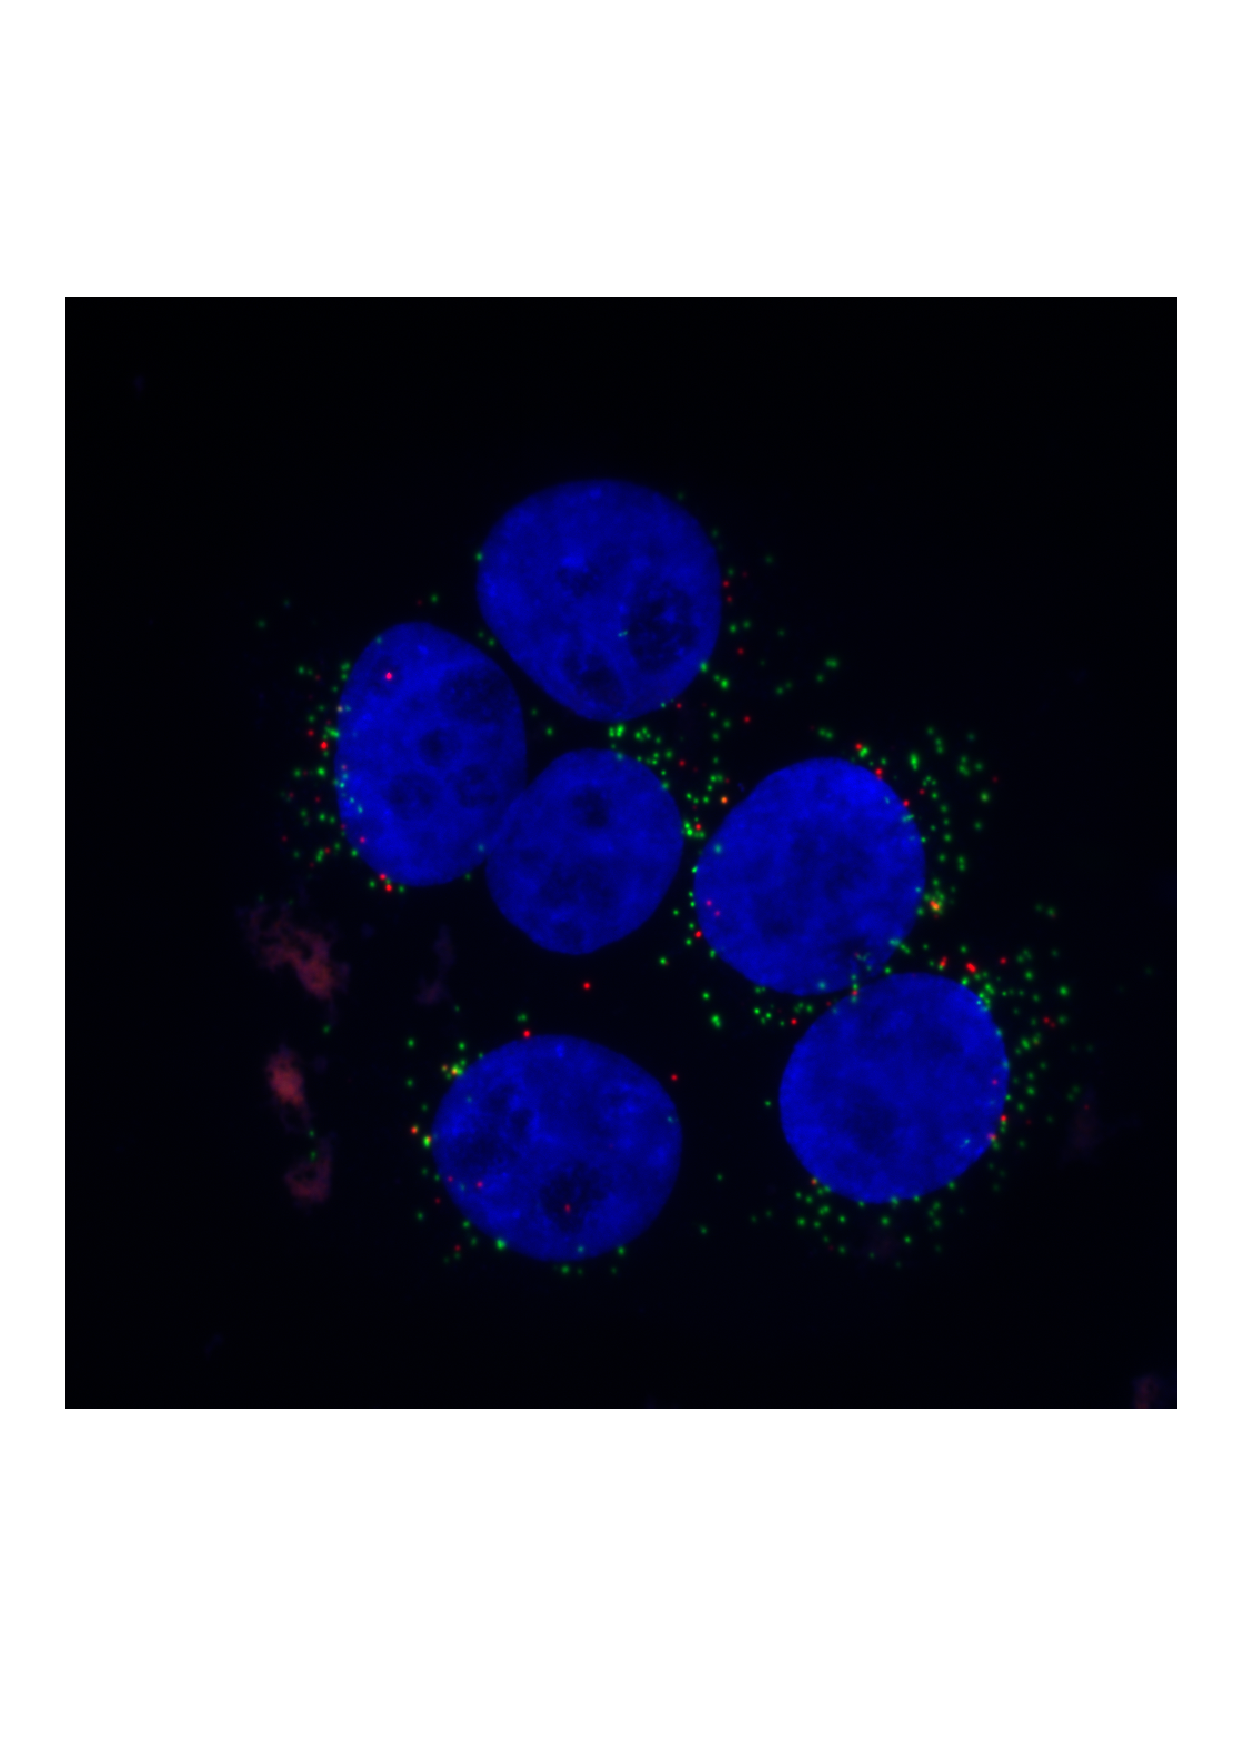
\includegraphics[width=0.3\textwidth]{Bilder/ImColour.pdf}
\caption{The original image.}
\label{fig:ImColour}
\end{figure}

\begin{figure}[ht]
\centering
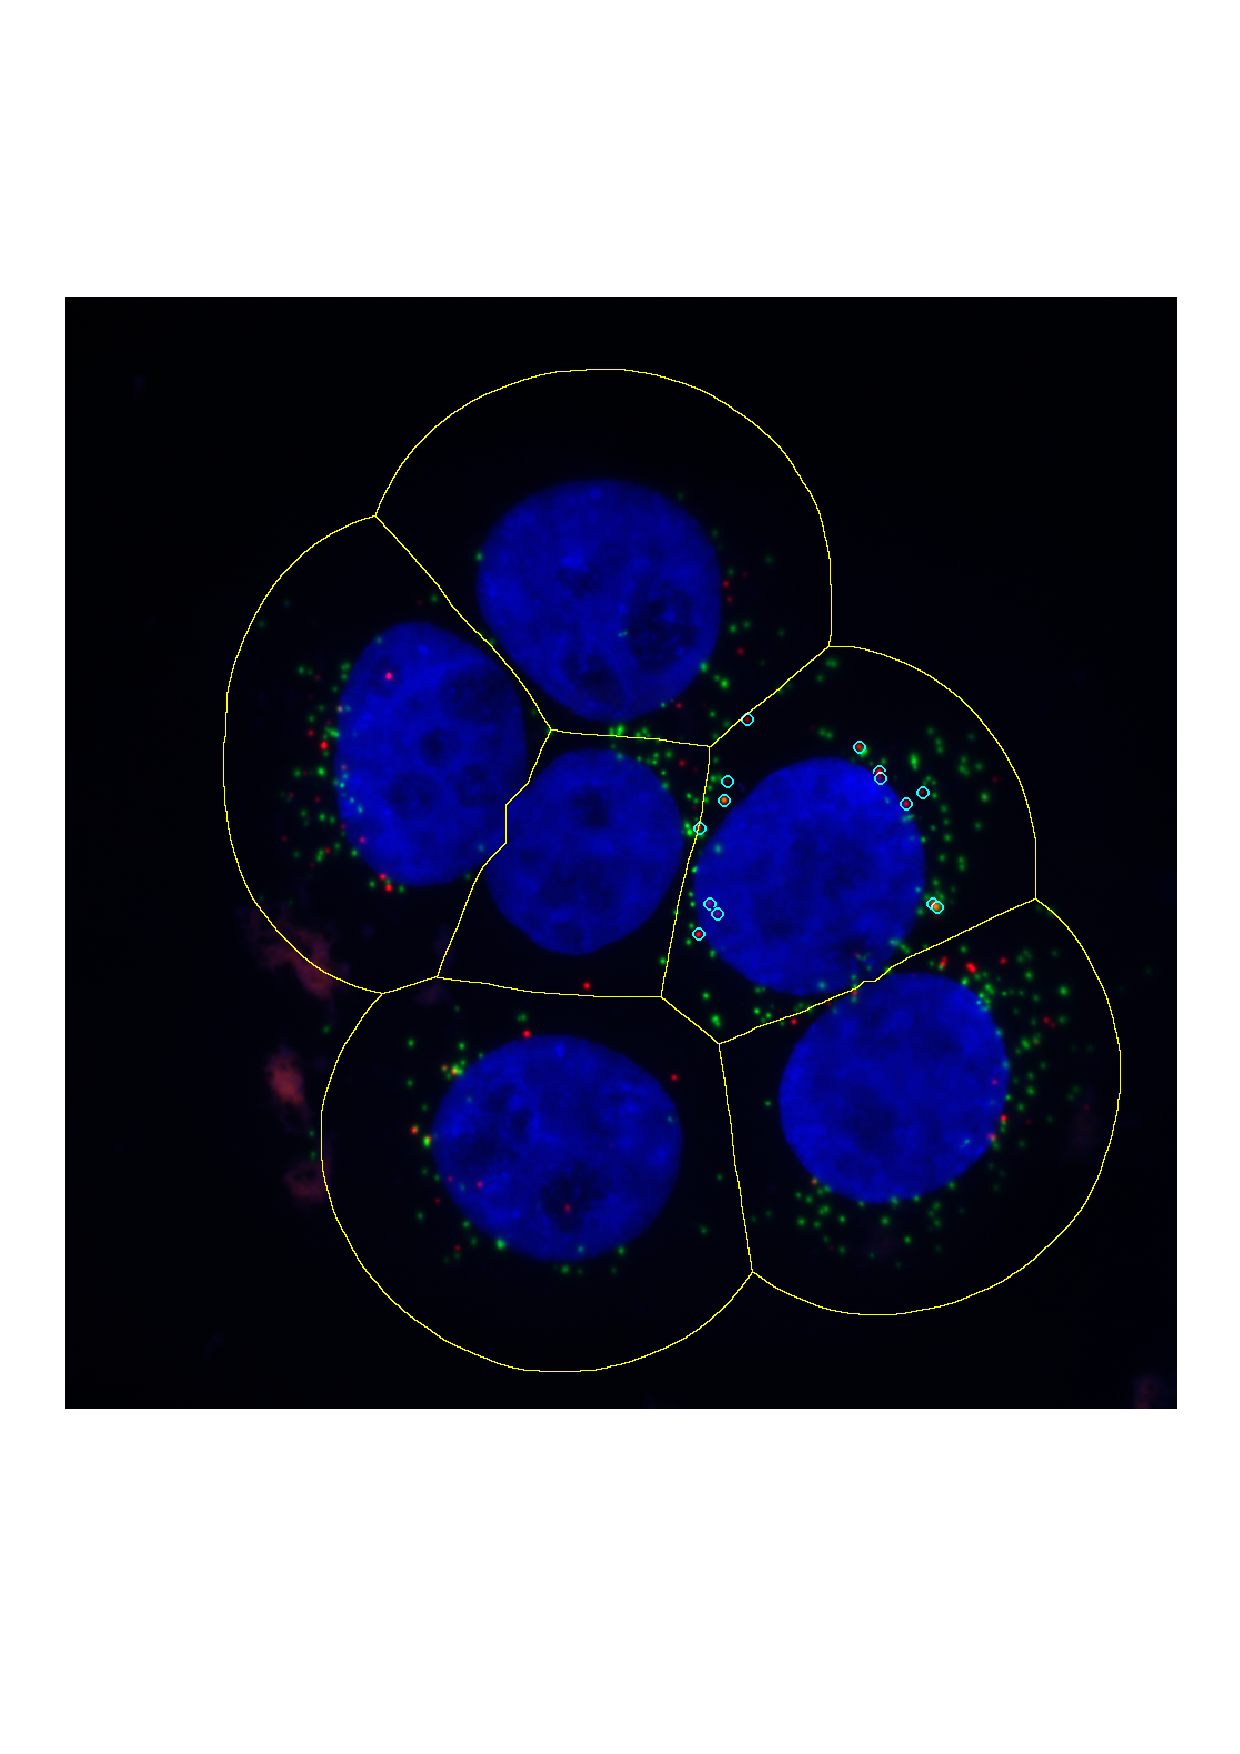
\includegraphics[width=0.3\textwidth]{Bilder/CellLinesNCircles.pdf}
\caption{The original image where cells have been segmented and padlock signals in cell nr 6 have been marked.}
\label{fig:CellLinesNCircles}
\end{figure}

\begin{figure}[ht]
\centering
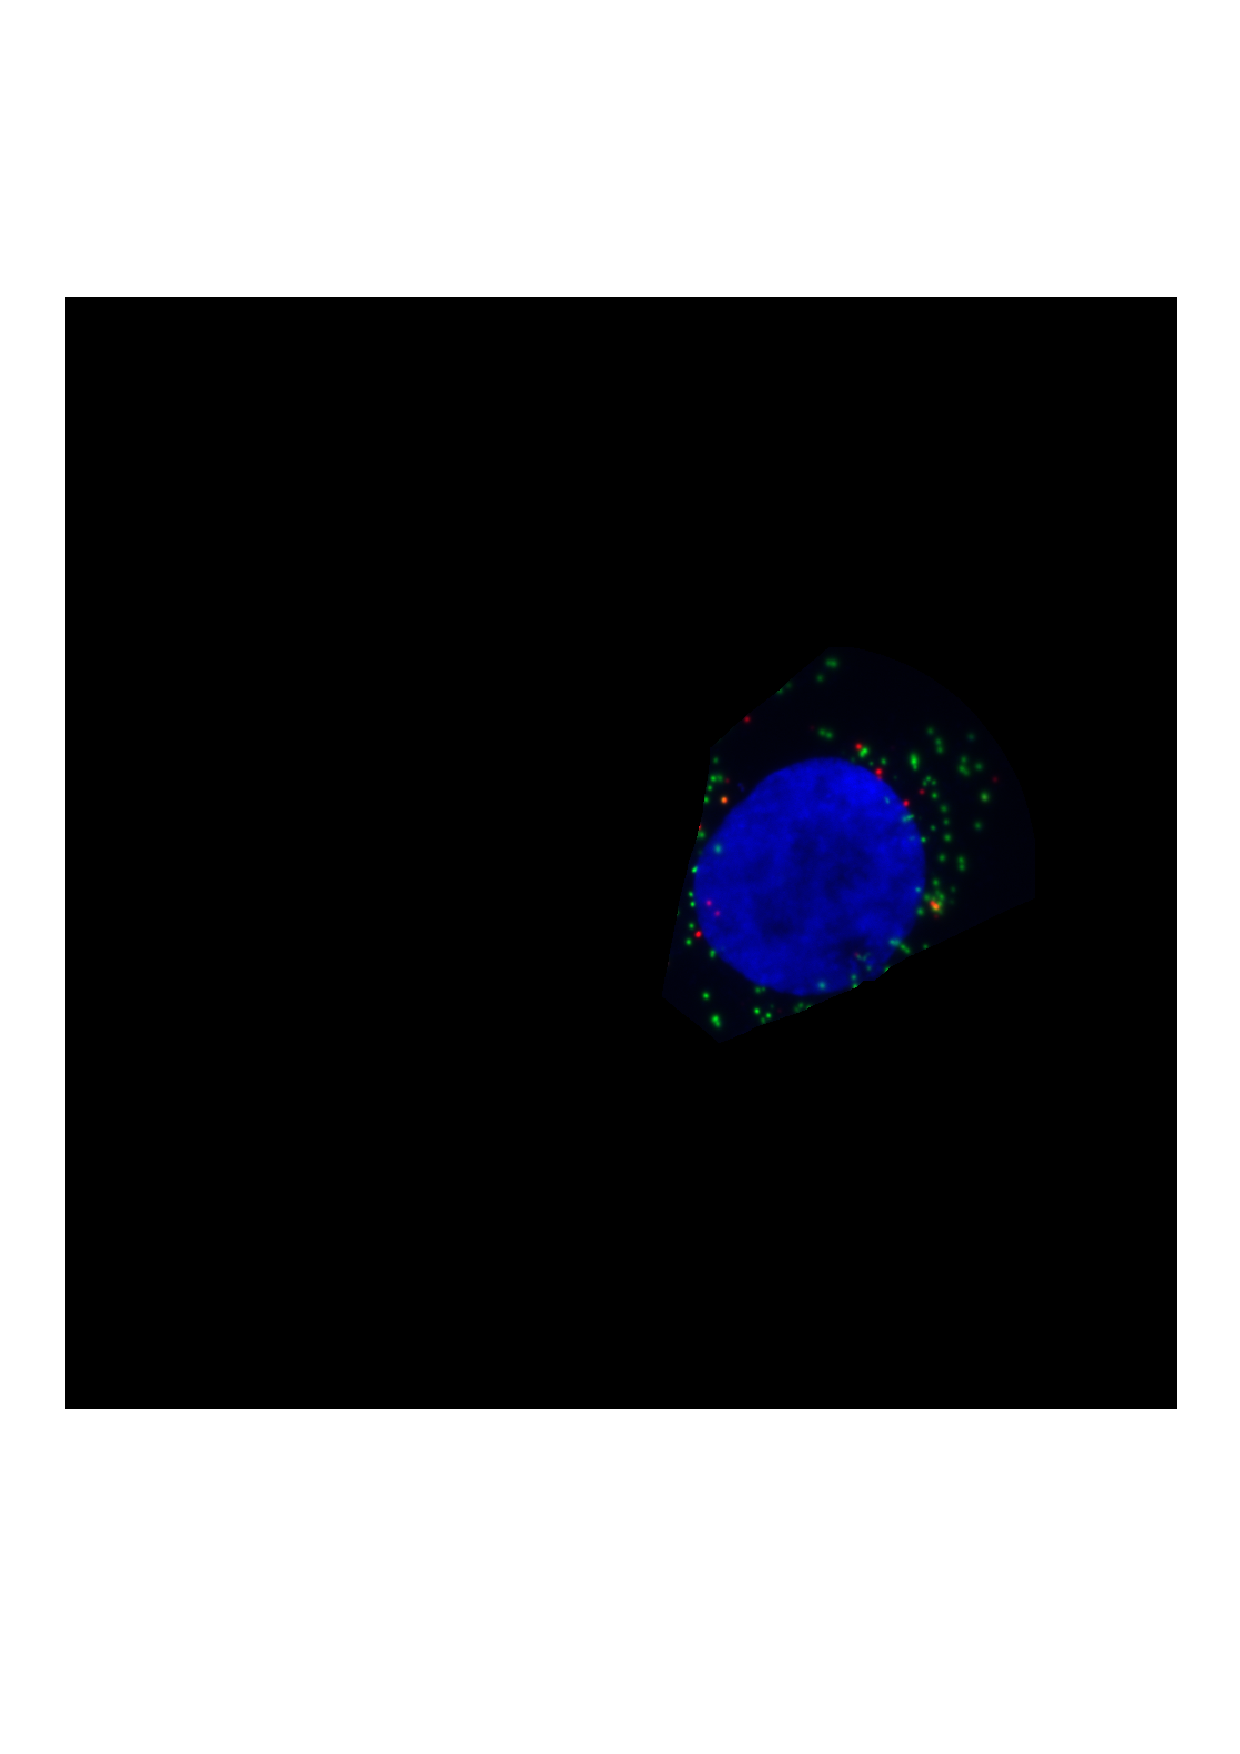
\includegraphics[width=0.3\textwidth]{Bilder/CellPart.pdf}
\caption{Cell nr 6 taken out of the original image.}
\label{fig:CellPart}
\end{figure}

%
%     WATERSHED SEGMENTATION
%

\section{Watershed segmentation 1} \label{sec:WatSeg1}
To get the image shown in figure \ref{fig:CellLinesNCircles}, segmentation
on the original image has to be done. To do so the first step is to get a binary image over the
six cell kernels. This is done by threshholding just the blue part(which represent the cell kernels)  of the original image. The threshold is determined by looking at
a histogram of that image. When the image is thresholded it still
contains some rubbish, see figure \ref{fig:CellKernelsThreshRough}. By performing
opening and closing the rubbish is removed and figure \ref{fig:CellKernelsThresSmooth} is received.

When a clean image over the cell kernels is made the watershed algorithm can be performed.
First a distance transform is made inside the objects, then the sign
of the distance transform is changed and the pixels outside the objects are set
to the minimum value, see figure \ref{fig:CellKernelsDist} and figure \ref{fig:CellKernelsDistInv}. All of the regional minimum values
are located and labeled. Figure \ref{fig:CellKernelsMinimum} is a close up off some of the regional minimums that are found.
The purpose of finding regional minimum values is to get one minumum value in each cell kernel so that
the watershed transform algorithm can be executed. As shown in figure \ref{fig:CellKernelsMinimum} there are
more then one minimum value in each kernel and also some "false minimum" inbetween kernels that are overlapping.
To get rid of these "false minimums" a demand on the depth of the minimum values are set. This removes some of the unwanted
minimums but there are still some extra minimums in the middle of the kernels. This
was solved by performing opening on the image which made the minimums in cell kernel centers close into a single shape,
see figure \ref{fig:CellKernelsMinimumOpened}.


\begin{figure}[ht]
\centering
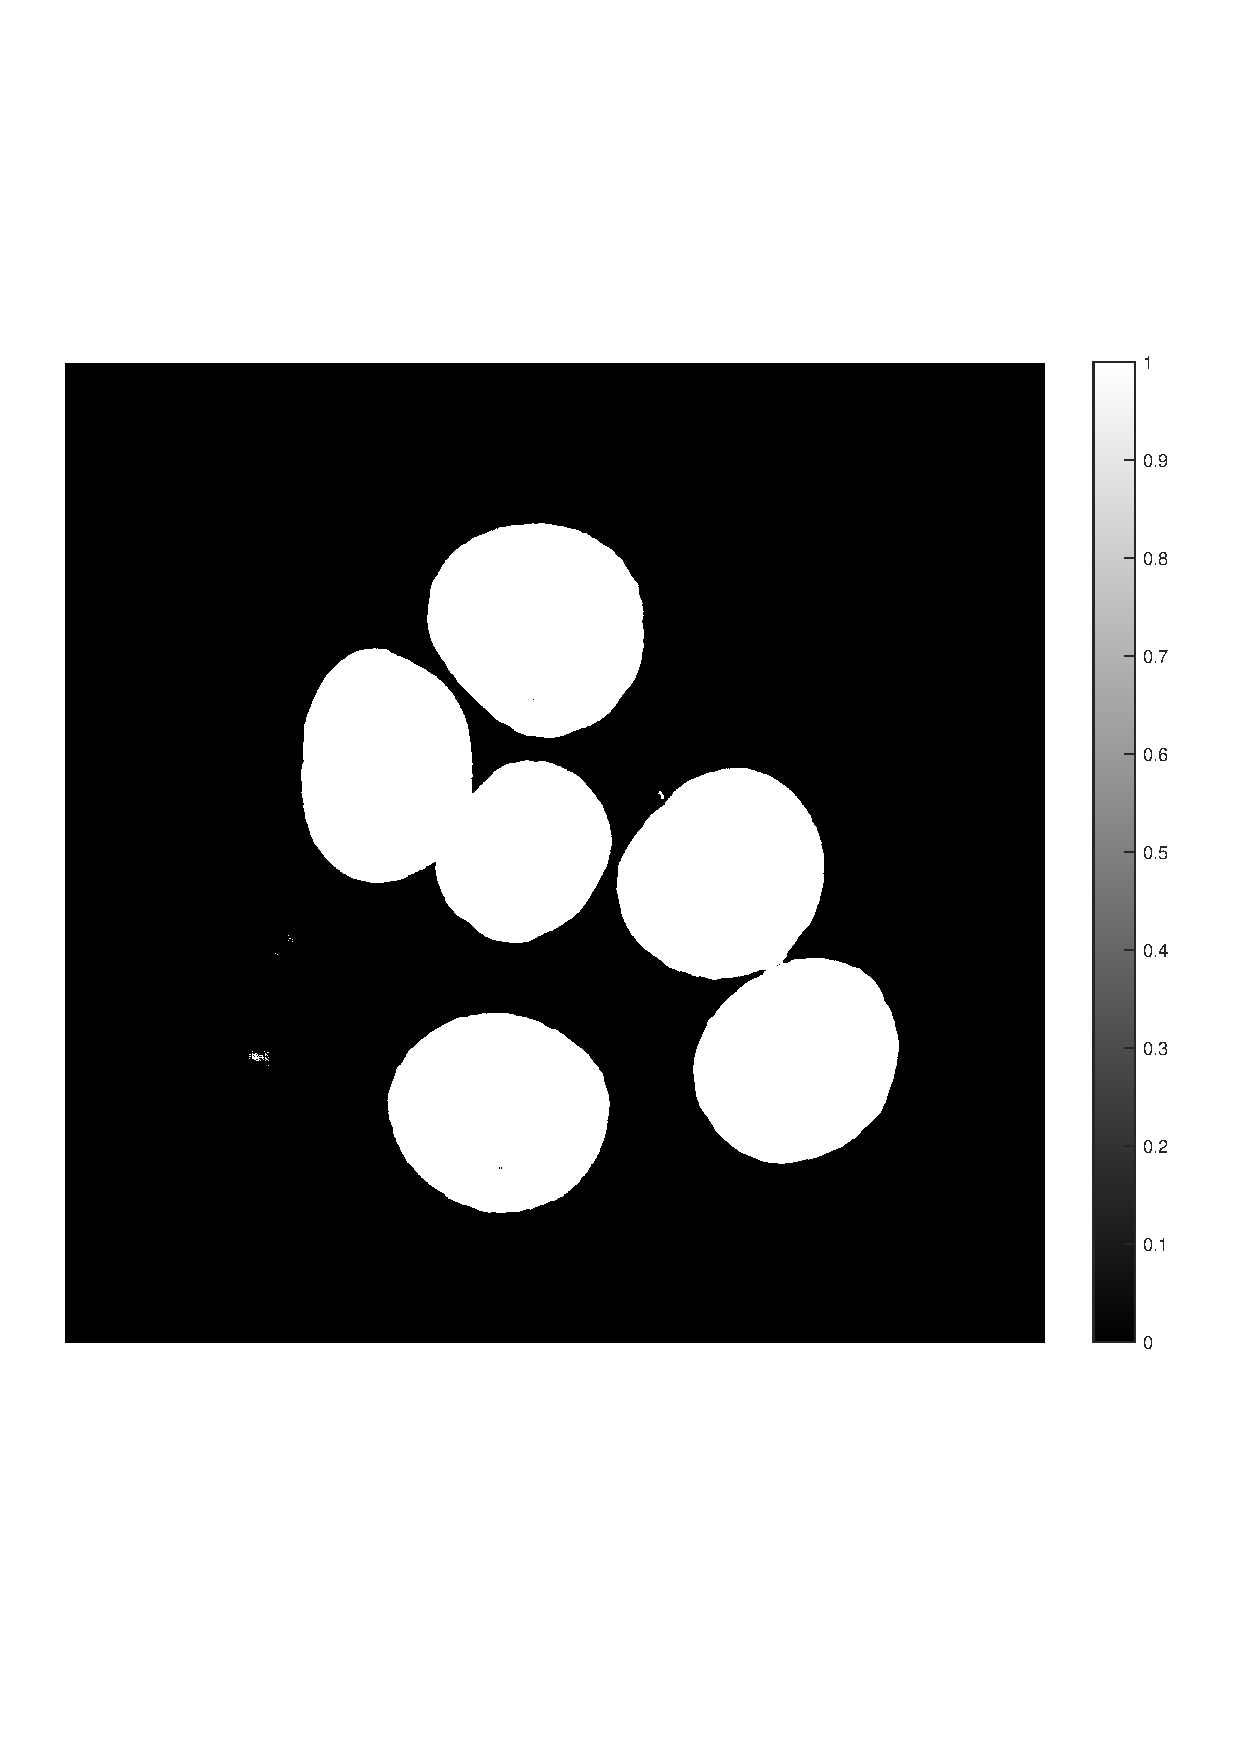
\includegraphics[width=0.3\textwidth]{Bilder/ThershholdedKernels.pdf}
\caption{A rough binary image of the cell kernels.}
\label{fig:CellKernelsThreshRough}
\end{figure}

\begin{figure}[ht]
\centering
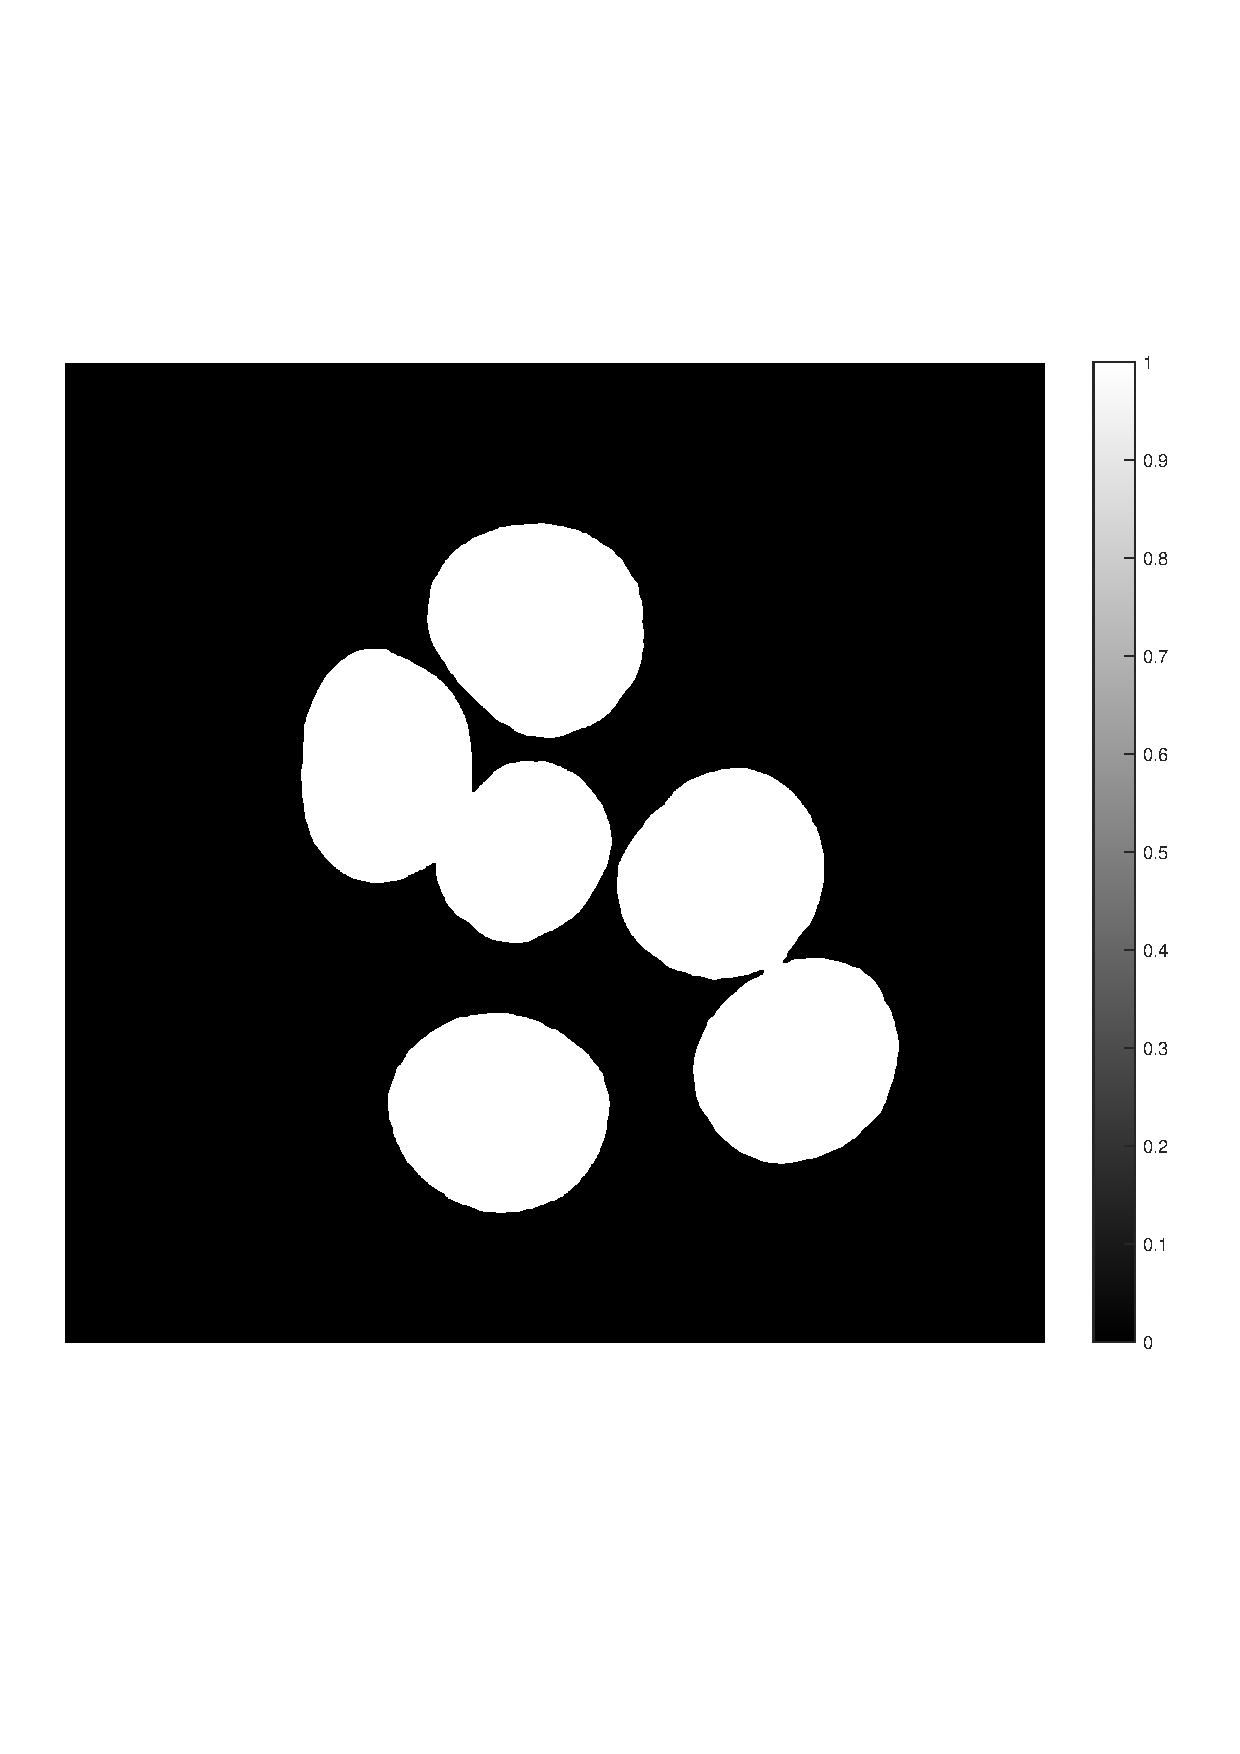
\includegraphics[width=0.3\textwidth]{Bilder/BWCleanKernels.pdf}
\caption{A smooth binary image of the cell kernels.}
\label{fig:CellKernelsThresSmooth}
\end{figure}

\begin{figure}[ht]
\centering
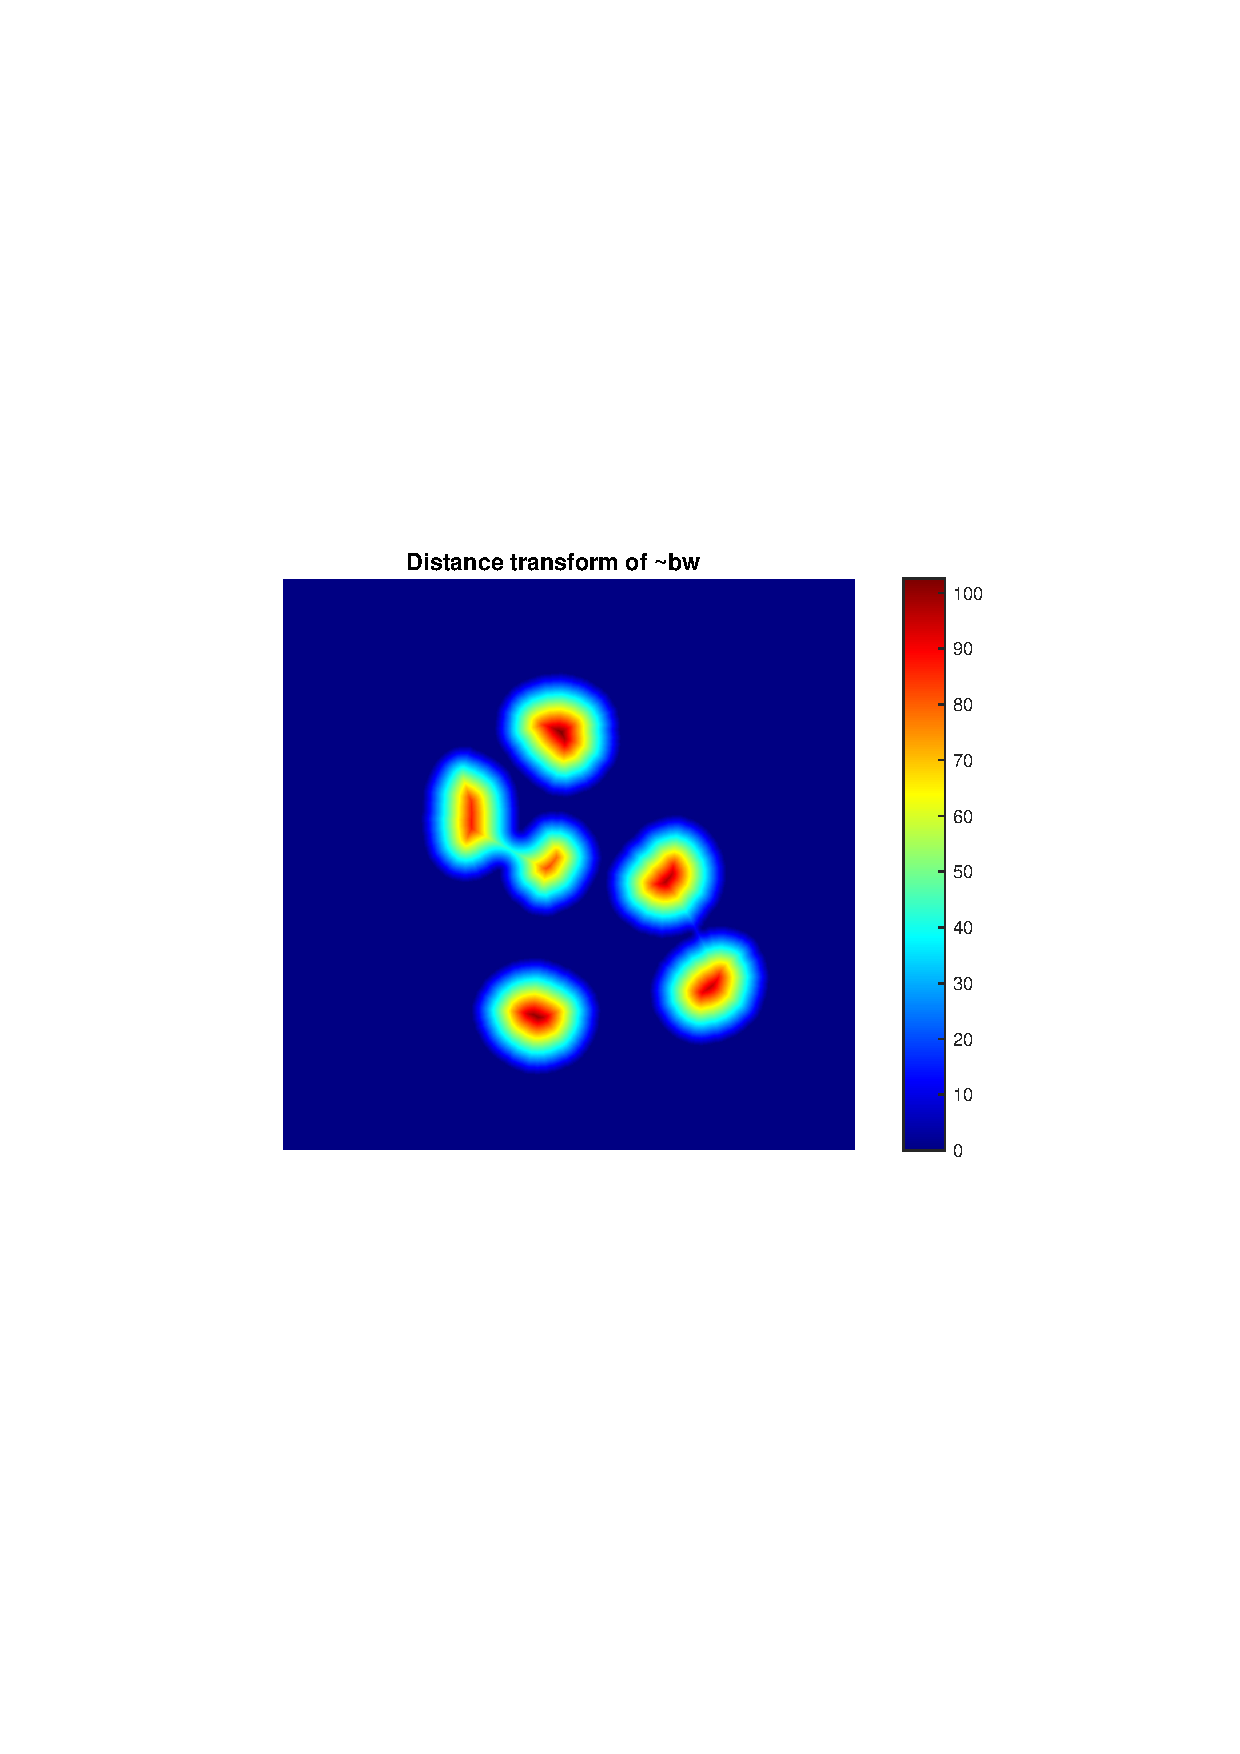
\includegraphics[width=0.6\textwidth]{Bilder/DistanceTransformInsideKernels.pdf}
\caption{A distancemap inside of the cell kernels.}
\label{fig:CellKernelsDist}
\end{figure}

\begin{figure}[ht]
\centering
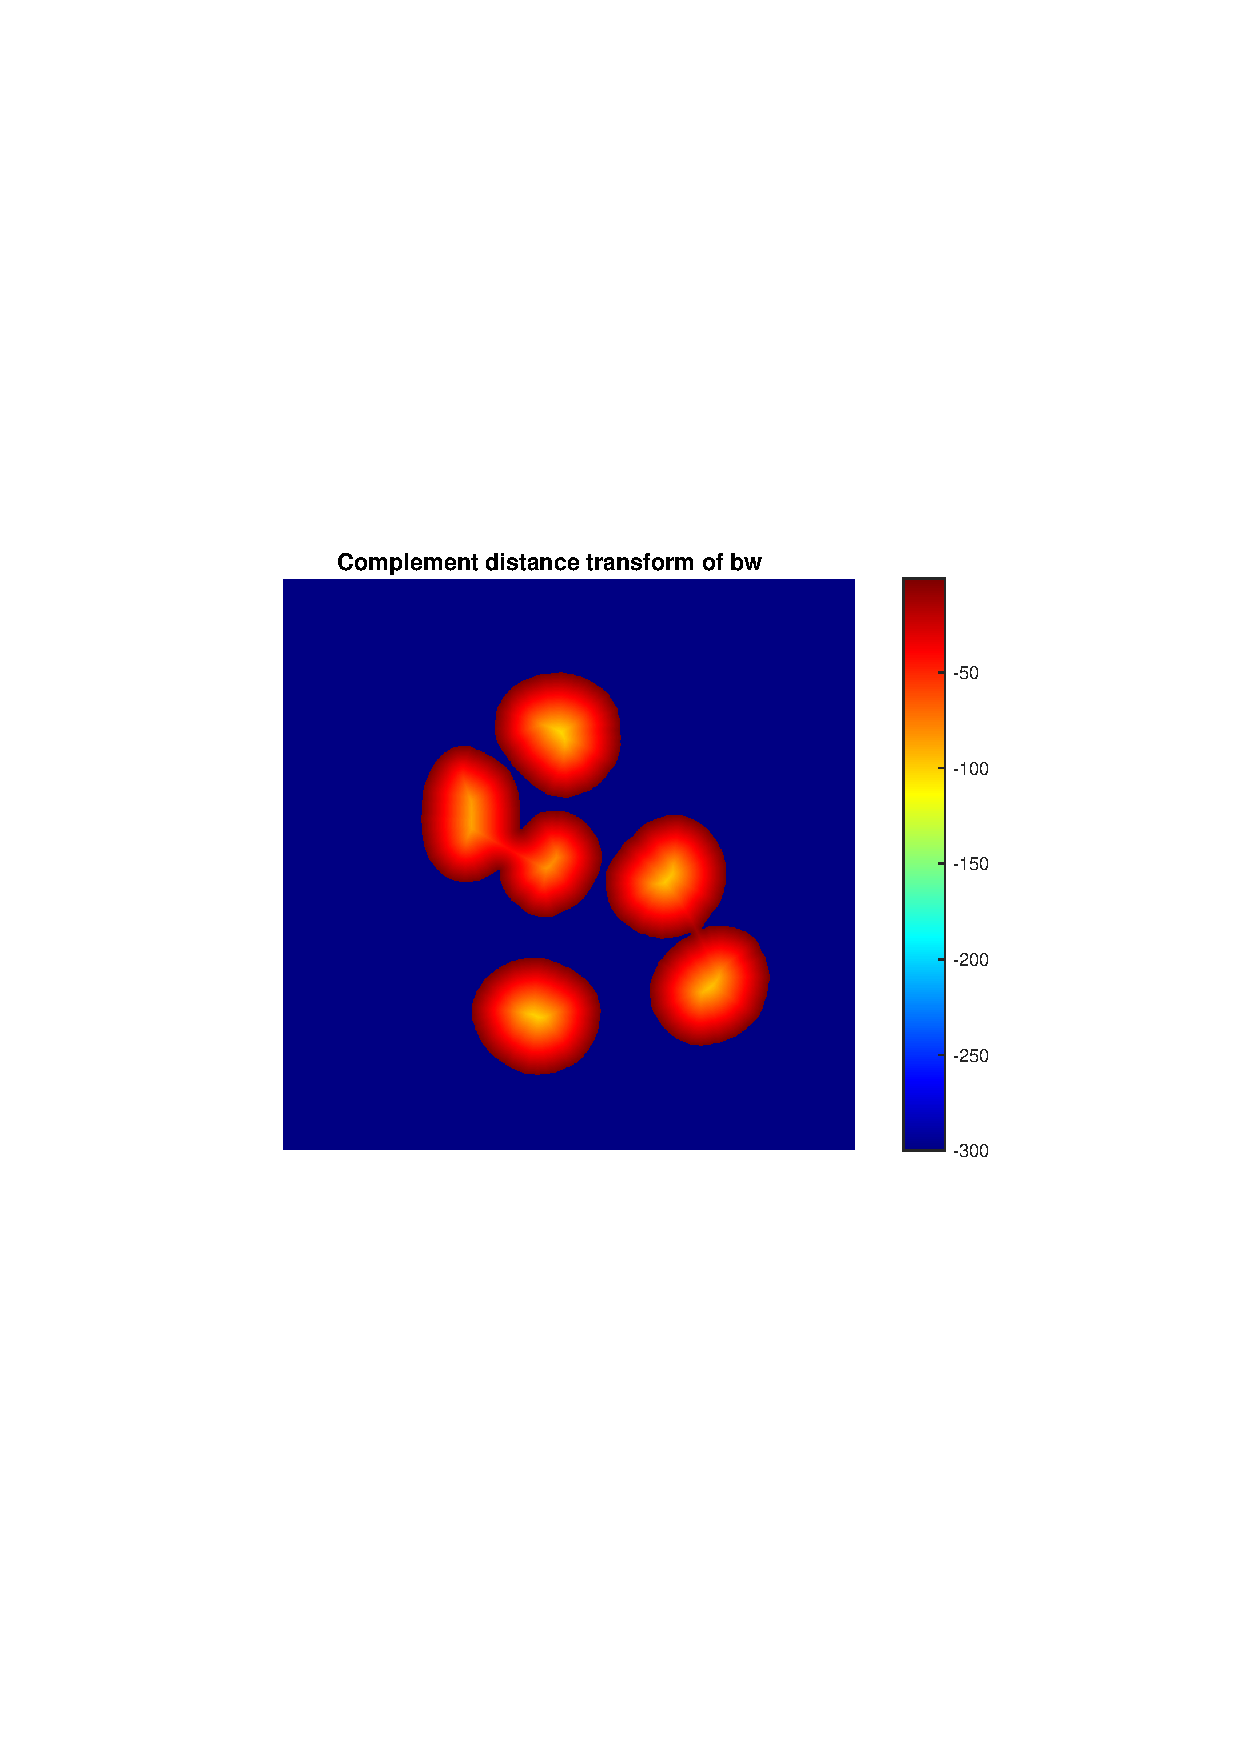
\includegraphics[width=0.6\textwidth]{Bilder/InvertedDistanceMap.pdf}
\caption{A inverted distancemap inside of the cell kernels.}
\label{fig:CellKernelsDistInv}
\end{figure}

\begin{figure}[ht]
\centering
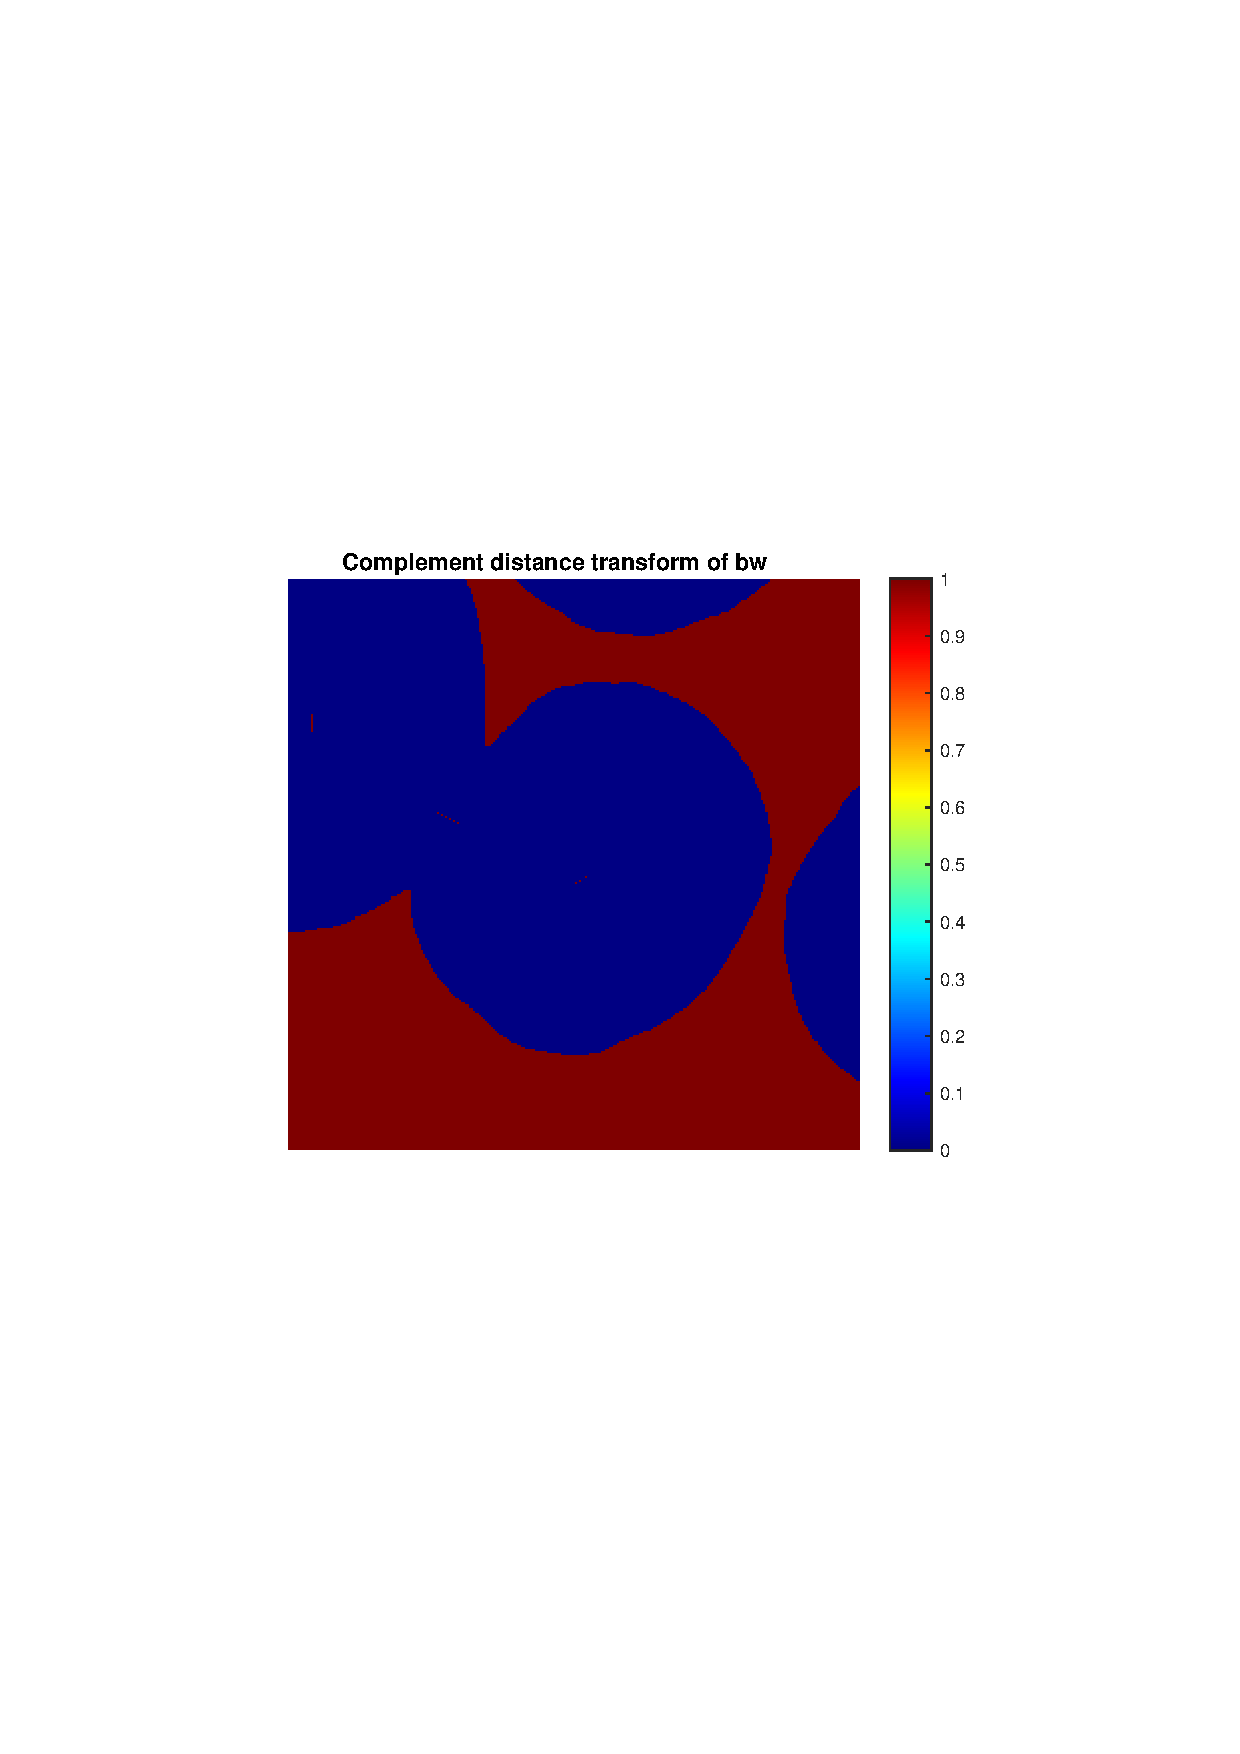
\includegraphics[width=0.6\textwidth]{Bilder/MinimumValusZoomedIn.pdf}
\caption{Some local minimus of the cell kernels.}
\label{fig:CellKernelsMinimum}
\end{figure}

\begin{figure}[ht]
\centering
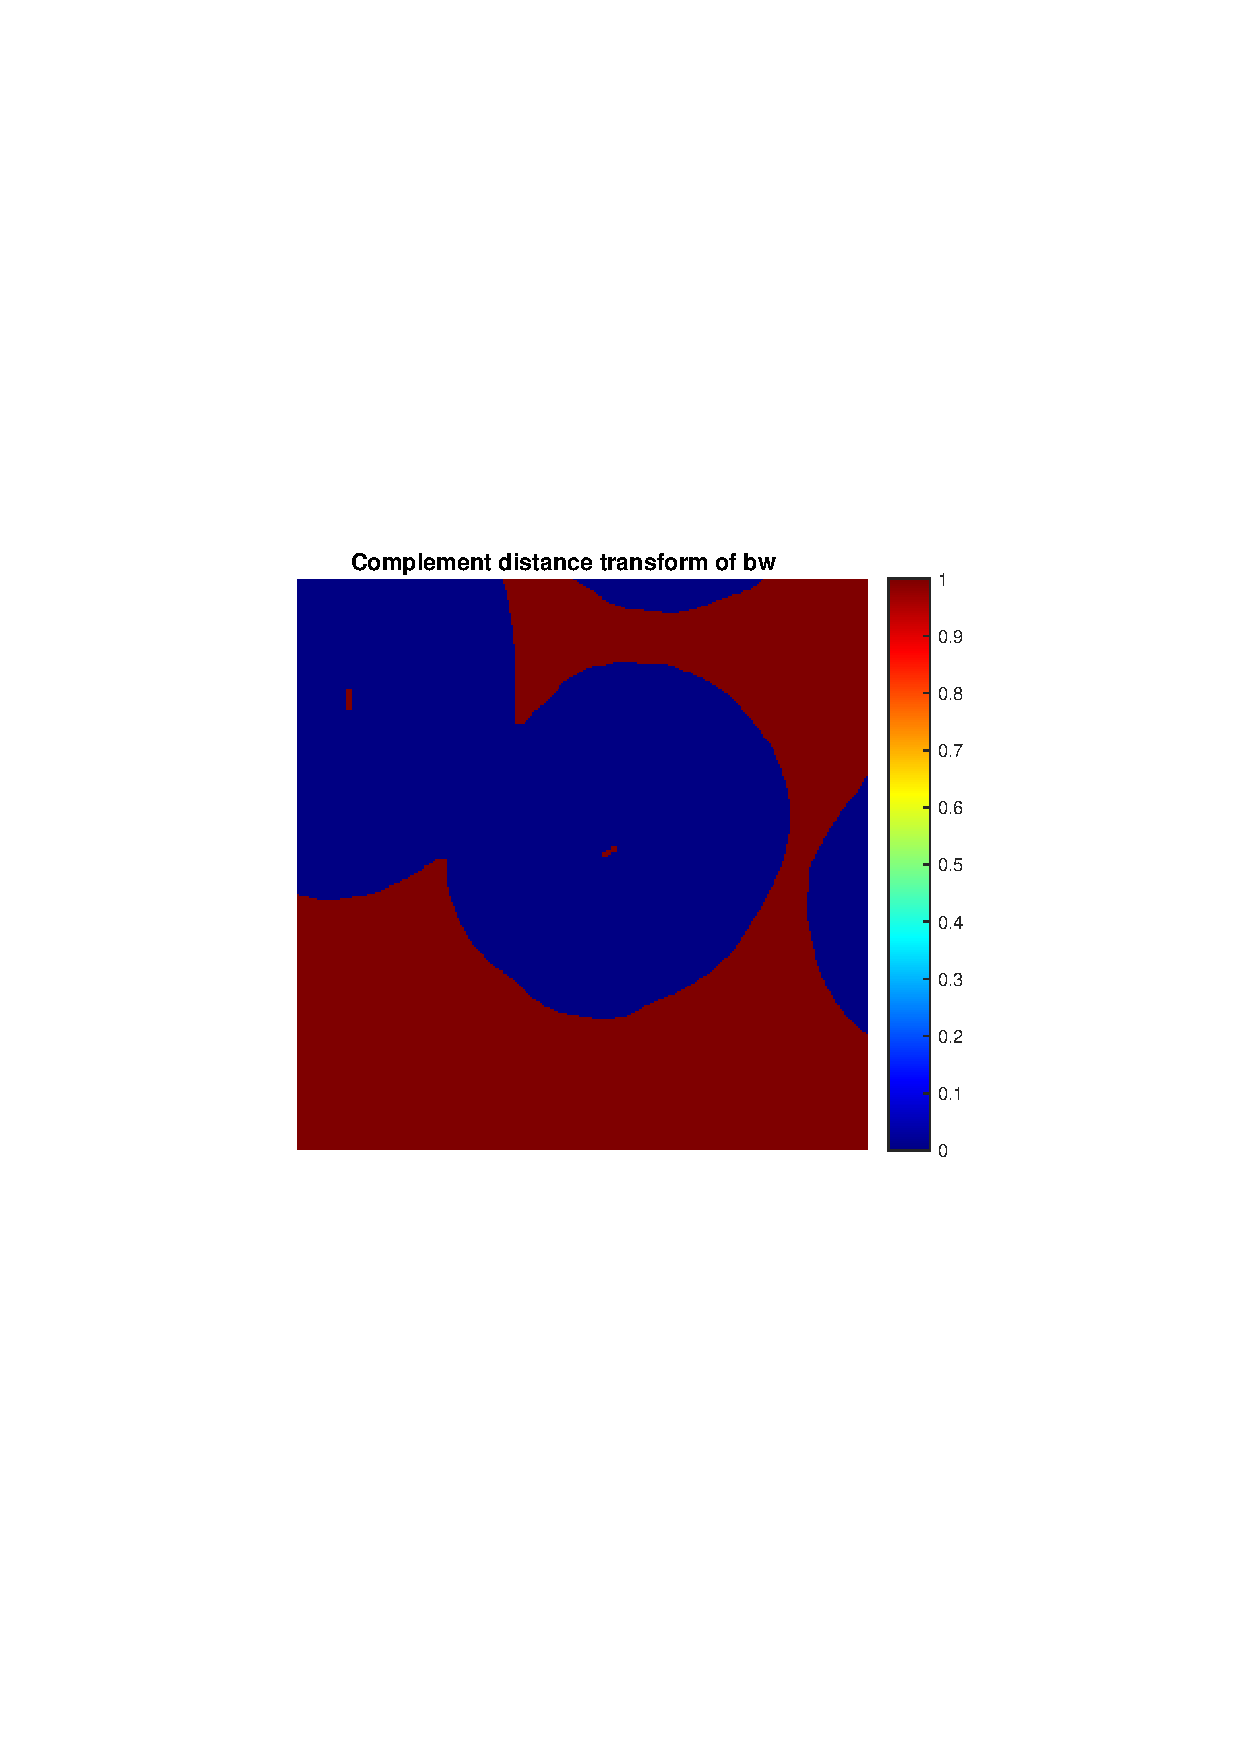
\includegraphics[width=0.6\textwidth]{Bilder/MinimumValesOpenedZoomedIn.pdf}
\caption{Some local minimus that have been opened.}
\label{fig:CellKernelsMinimumOpened}
\end{figure}

\section{Watershed segmentation 2}
In order to get a properly segmented image over the cell kernels with the
surrounding cytoplasm we start with the binary image shown in figure \ref{fig:CellKernelsThresSmooth}. Then preform a
simular watershed algorithm as in section \ref{sec:WatSeg1}. First a distance
map is performed outside of the cell kernels, see figure \ref{fig:CellDist}. Then the distance map is
inverted and values lower then a threshold is set to that threshold.
Thresholding it and removing the cell kernels then gives figure \ref{fig:CellBWMask}.
Removing the cell kernels from the center of the image is done in order to create centers for the
watershed algorithm to begin "filling" water. Before the watershed algorithm can
be applied the different centers need to be labeled, see figure \ref{fig:CellCyto}.
After labeling, the watershed algorithm can be used, resulting in figure \ref{fig:CellLabeled}.
From which the binary image shown in figure \ref{fig:CellBw} can be created.

\begin{figure}[ht]
\centering
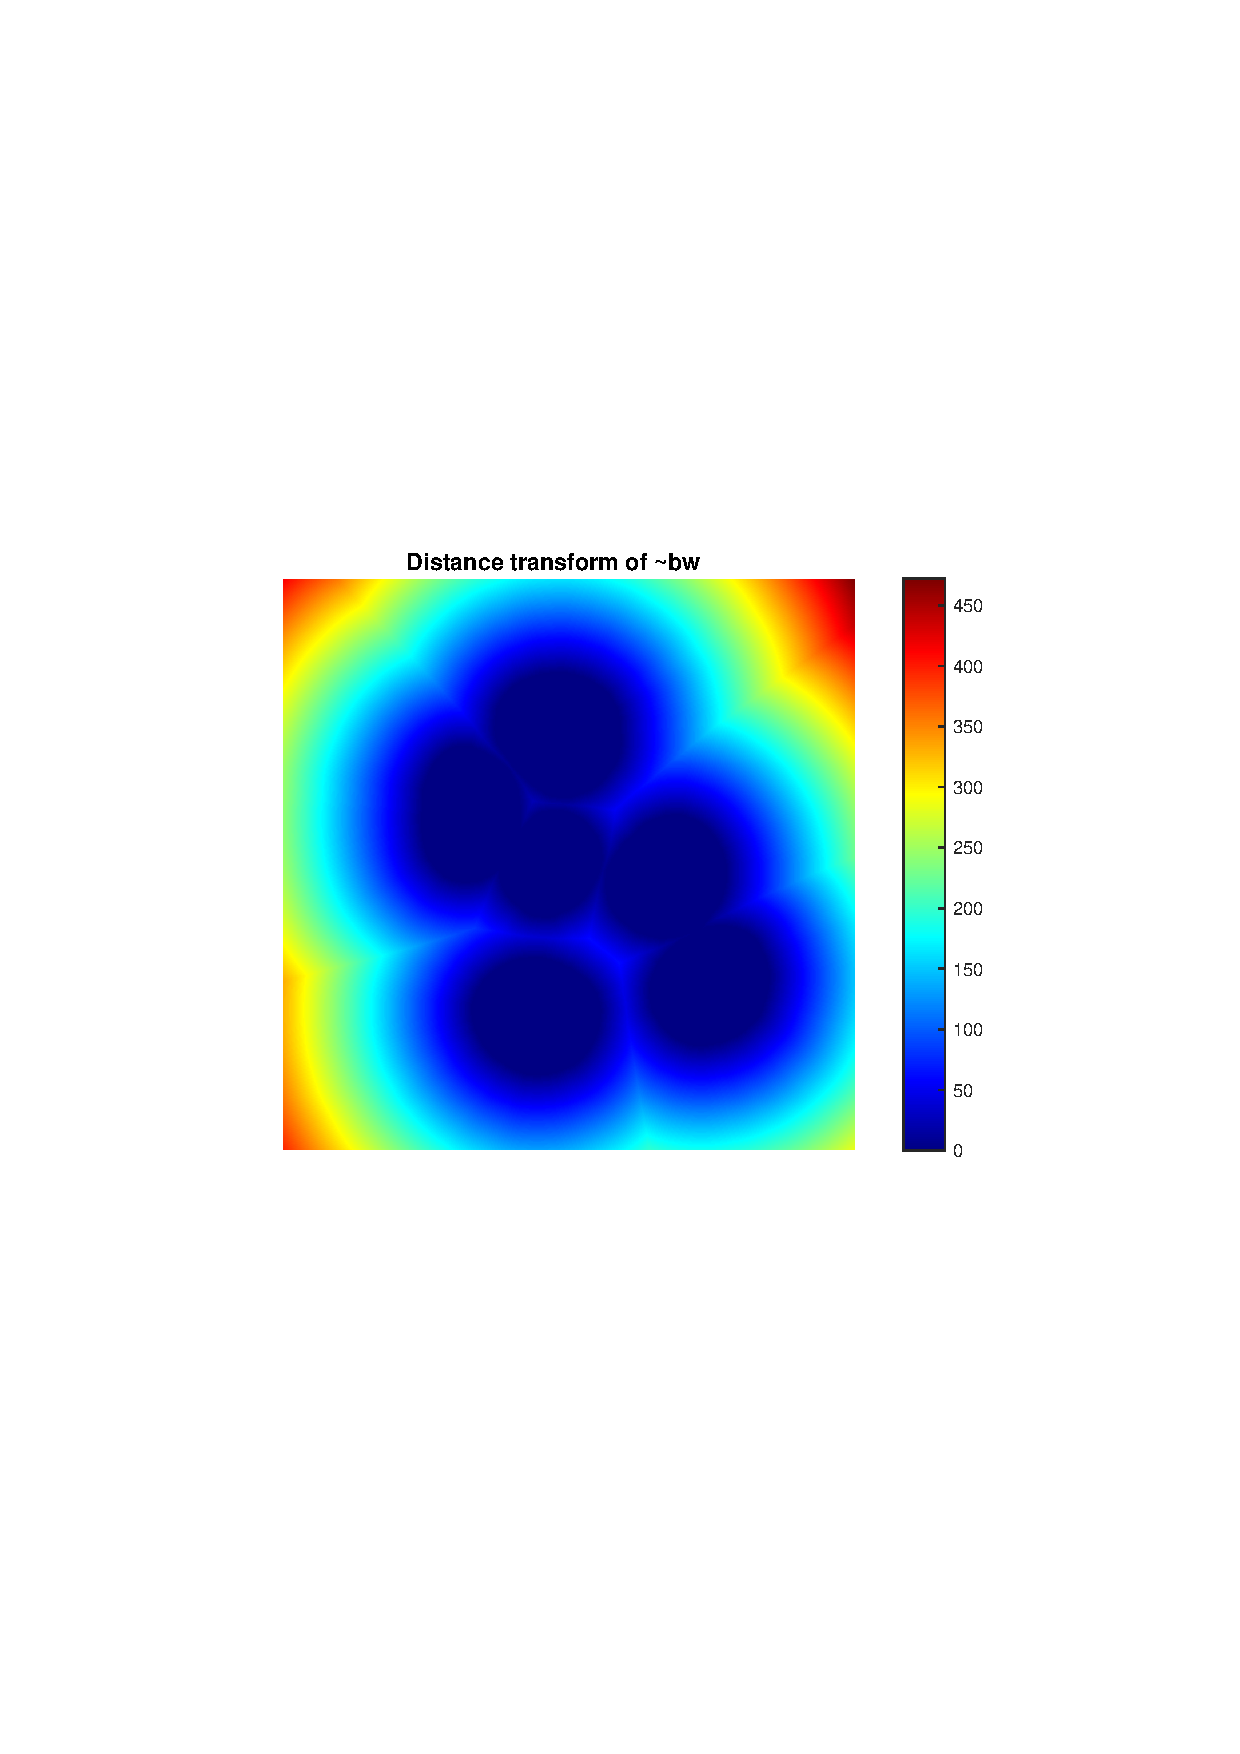
\includegraphics[width=0.6\textwidth]{Bilder/CellDist.pdf}
\caption{Distance map outside cell kernel.}
\label{fig:CellDist}
\end{figure}

\begin{figure}[ht]
\centering
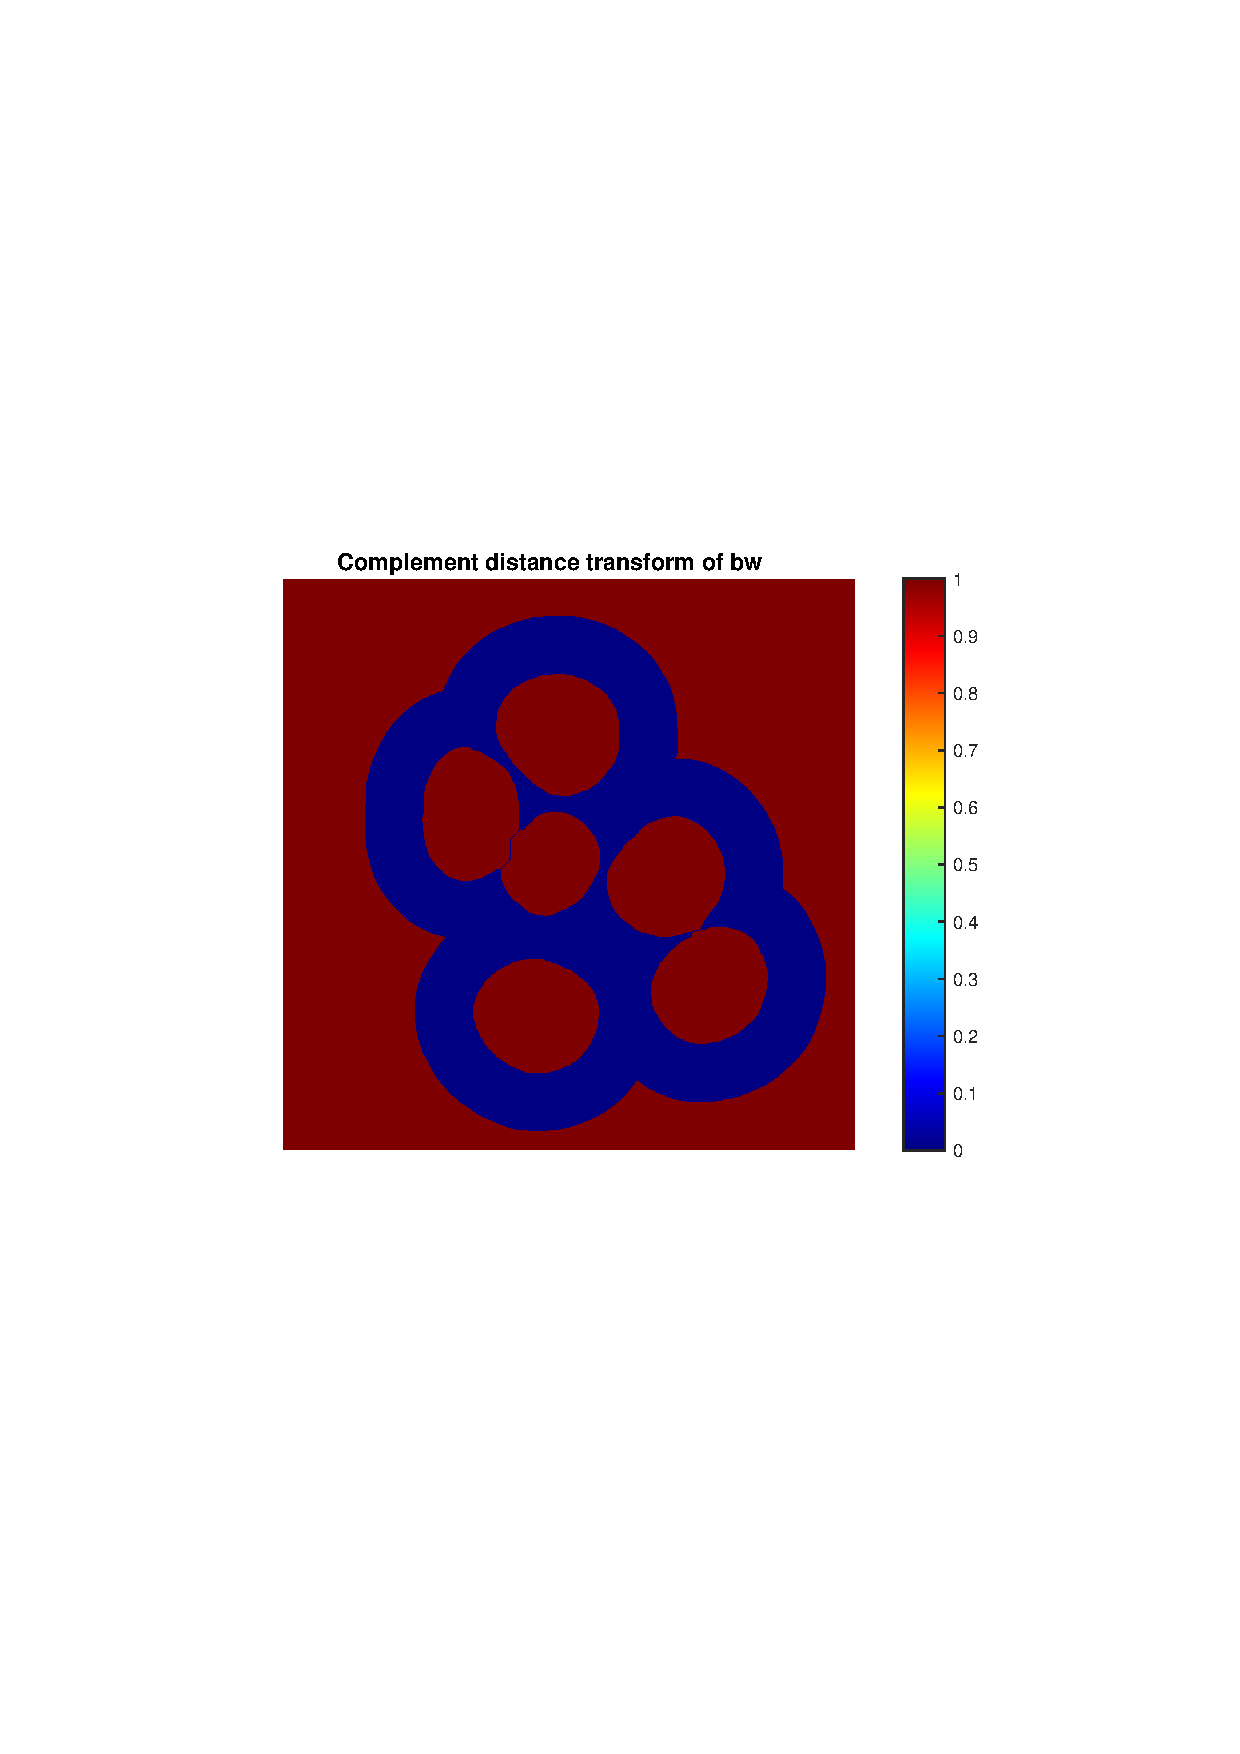
\includegraphics[width=0.6\textwidth]{Bilder/CellBwMask.pdf}
\caption{Binary cell cytoplasma.}
\label{fig:CellBWMask}
\end{figure}

\begin{figure}[ht]
\centering
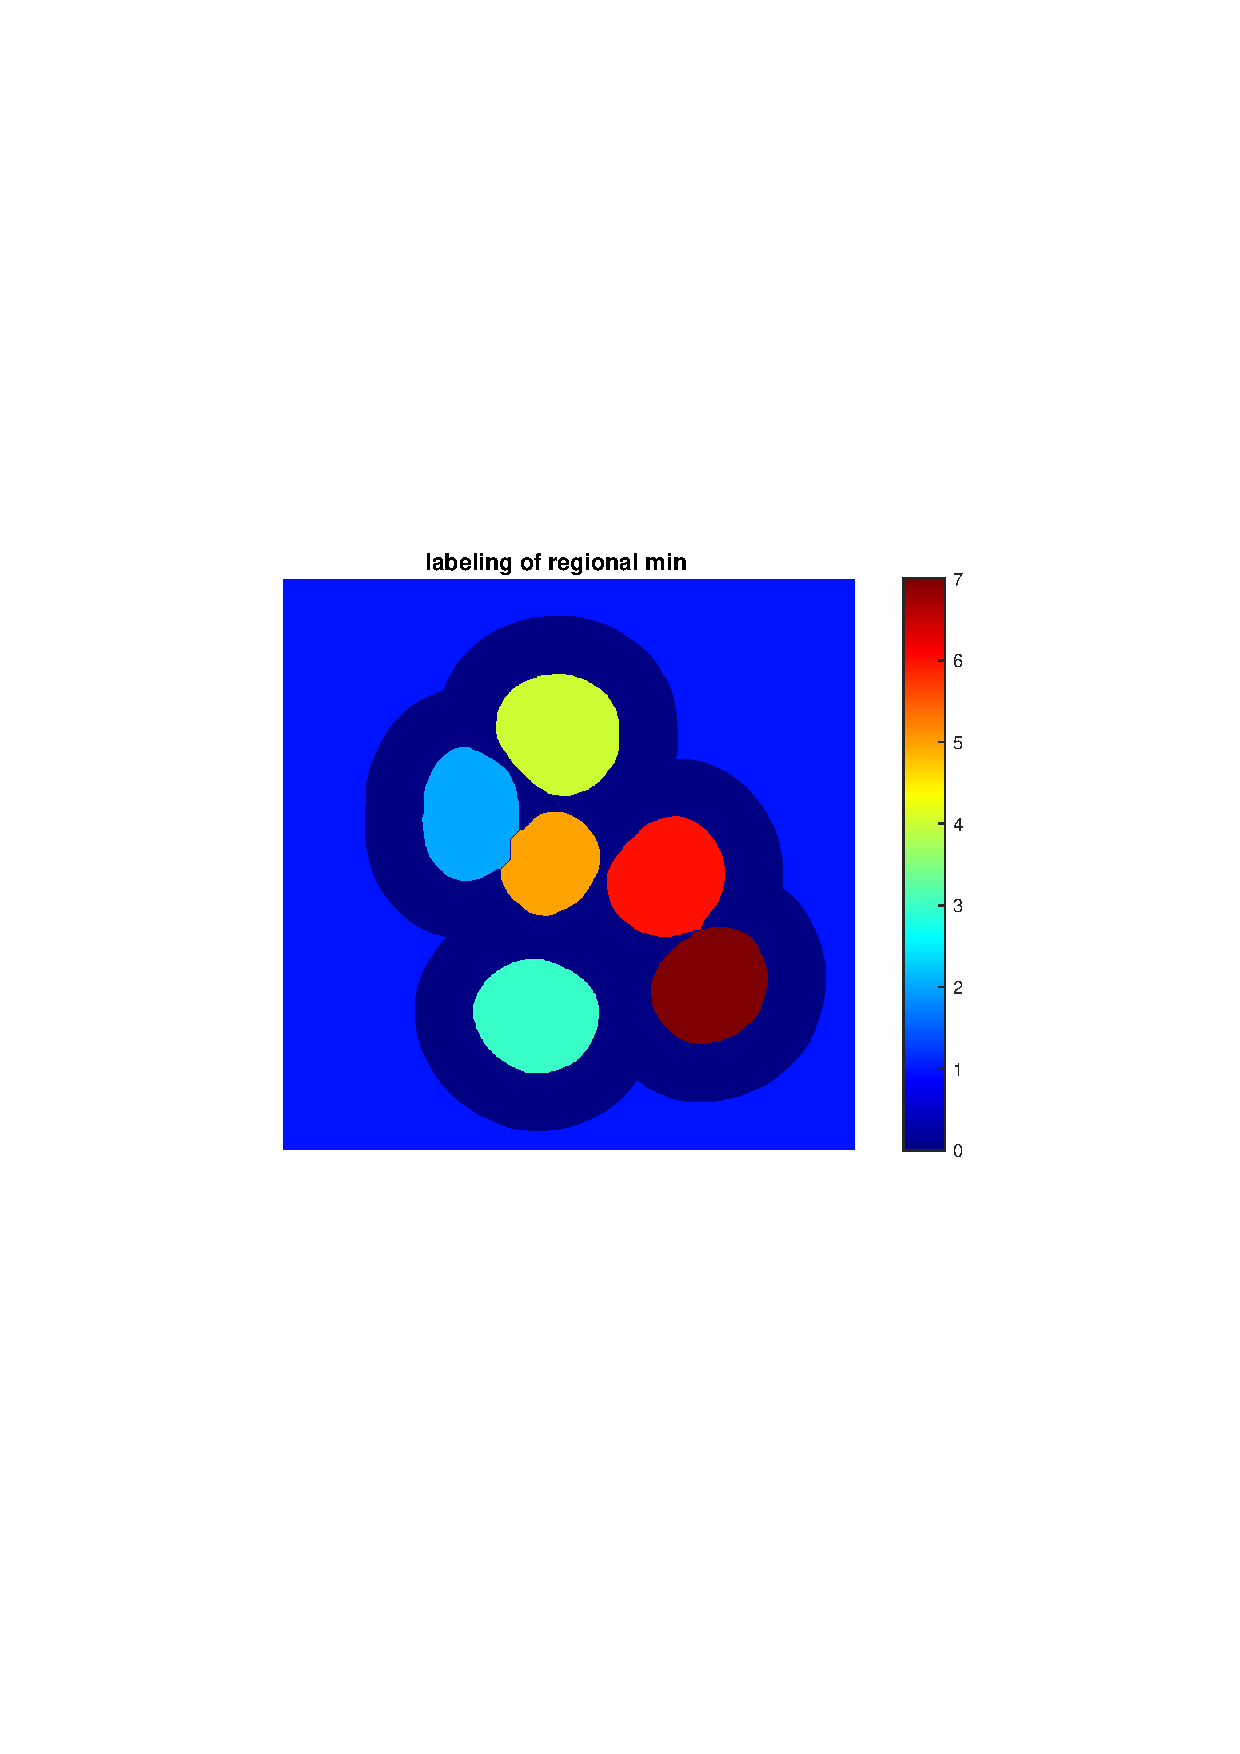
\includegraphics[width=0.6\textwidth]{Bilder/CellBwLabeldKernels.pdf}
\caption{Cell kernels labeled with cytoplasma area marked.}
\label{fig:CellCyto}
\end{figure}

\begin{figure}[ht]
\centering
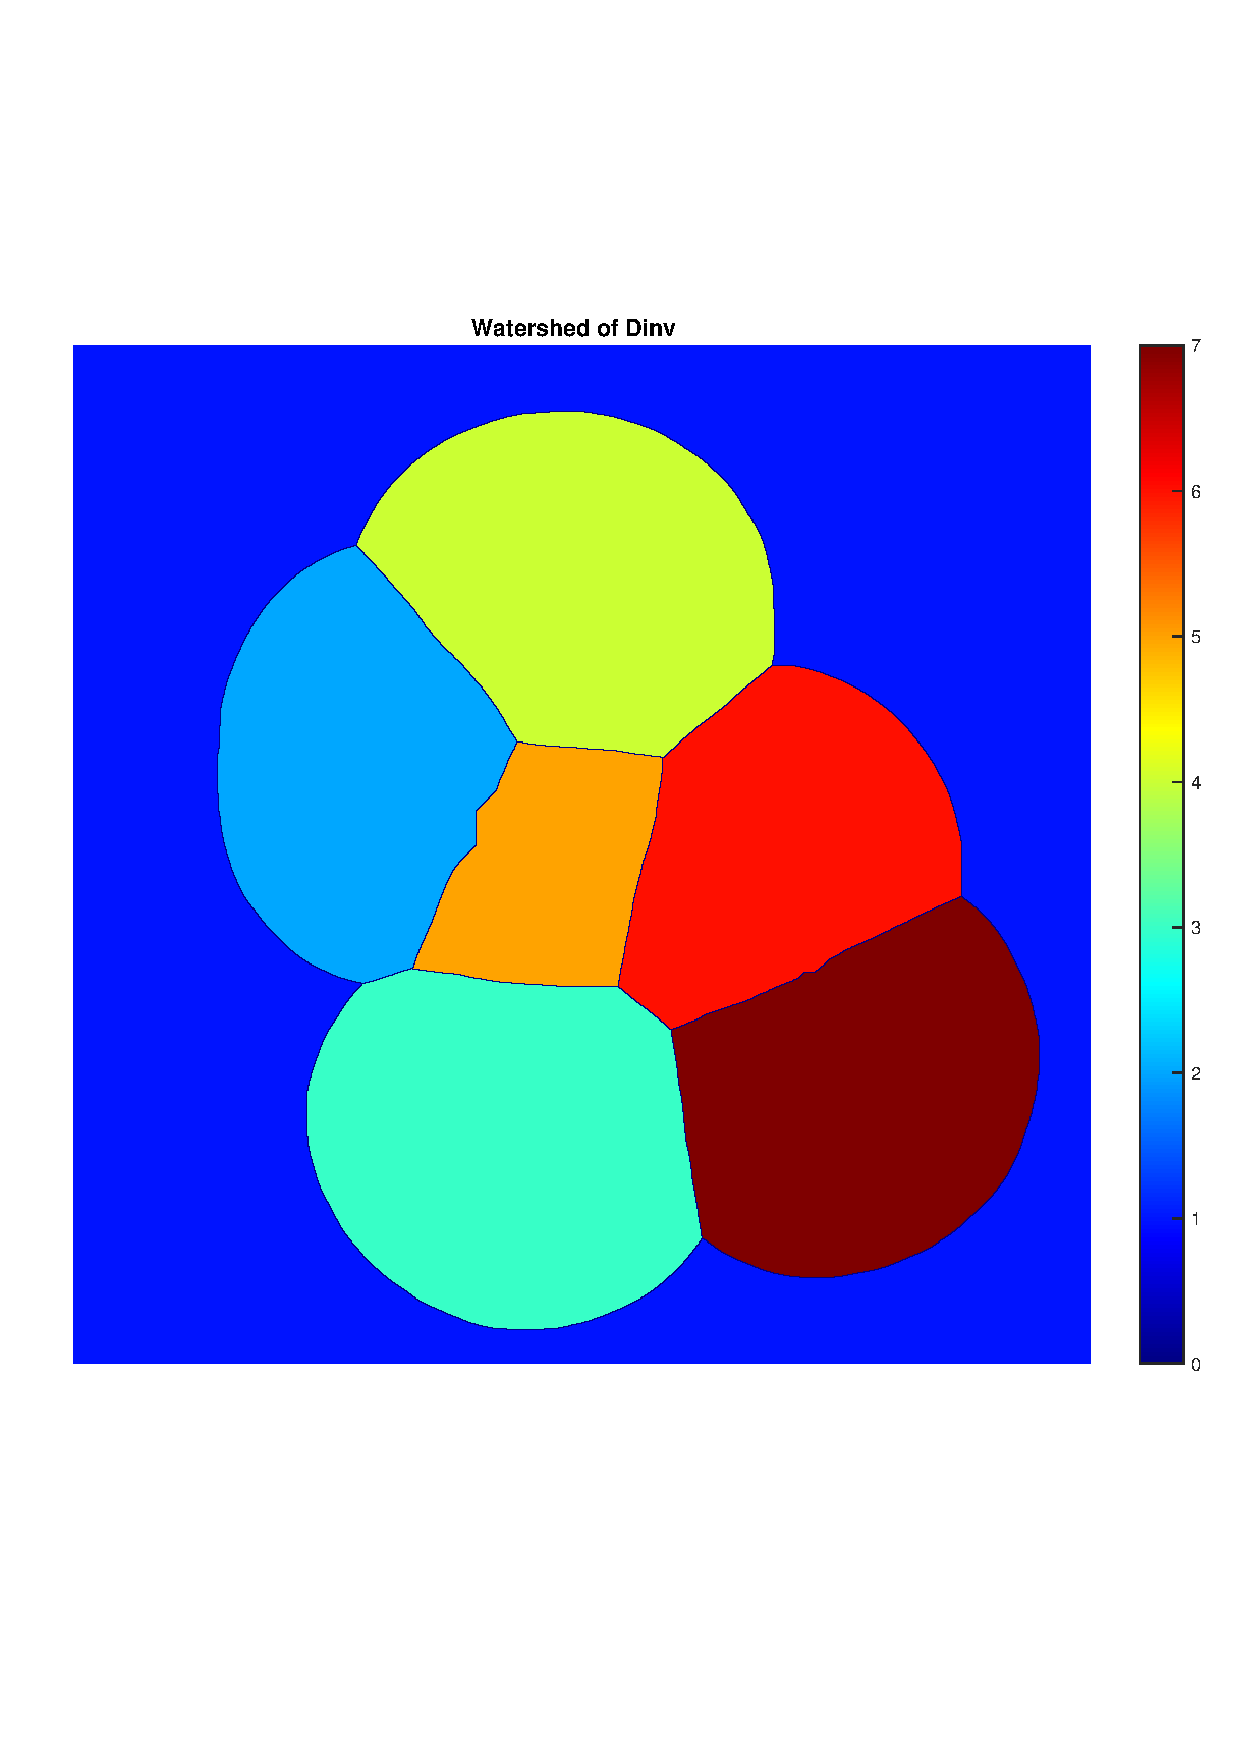
\includegraphics[width=0.3\textwidth]{Bilder/CellBwLabeld.pdf}
\caption{Labeled cells.}
\label{fig:CellLabeled}
\end{figure}

\begin{figure}[ht]
\centering
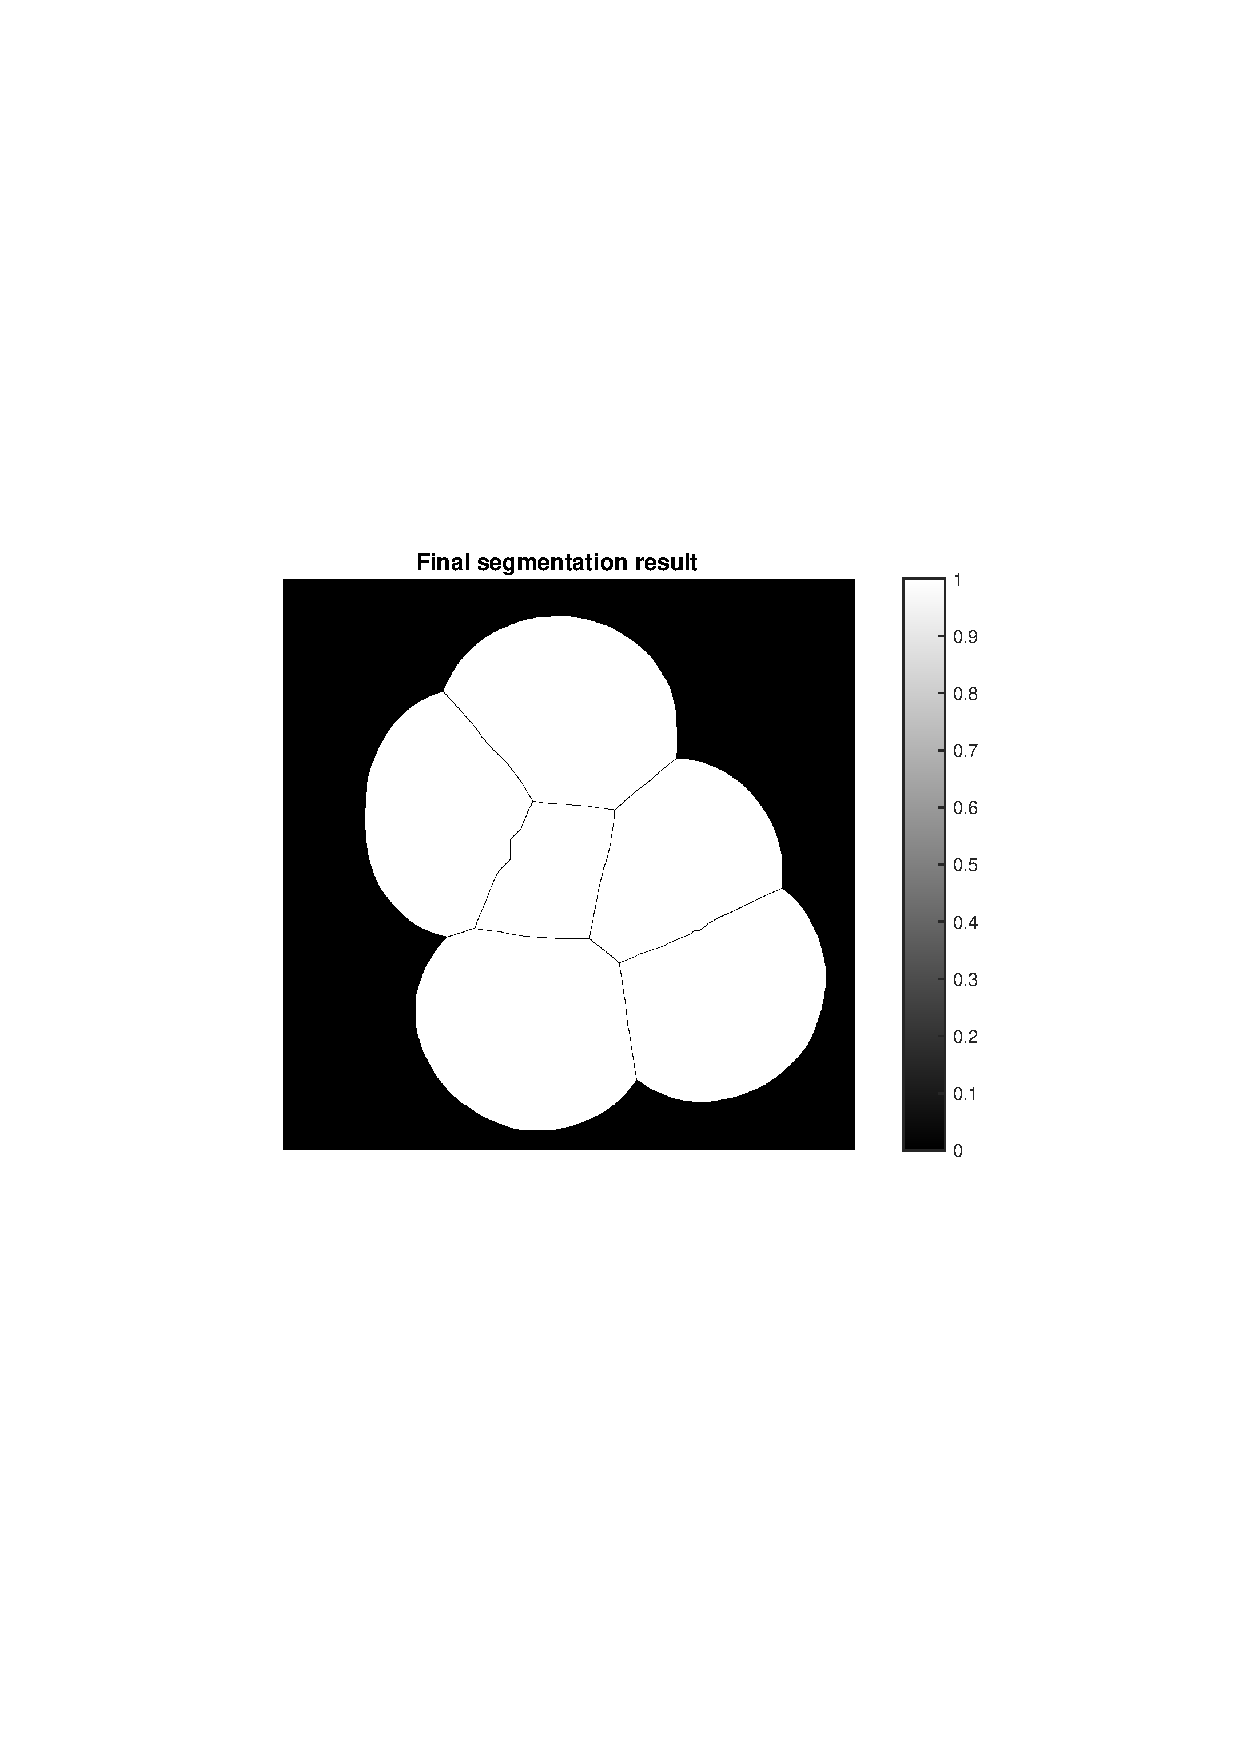
\includegraphics[width=0.6\textwidth]{Bilder/CellBw.pdf}
\caption{Binary cells.}
\label{fig:CellBw}
\end{figure}

\section{Outlining cytoplasm}
Getting the pixels representing the borders between different cells cytoplasma can
easily be done be taking out the pixels with value zero from figure \ref{fig:CellLabeled}.
These pixels are then colored yellow, see figure \ref{fig:CellLines}.
By taking out the pixels representing cell kernel and cell cytoplasm 6 from figure
\ref{fig:ImColour}, figure \ref{fig:CellPart} is created. The 14 padlock signals can then be located and marked with cyan cirkels, resulting in the finished image shown in figure \ref{fig:CellLinesNCircles}.

\begin{figure}[ht]
\centering
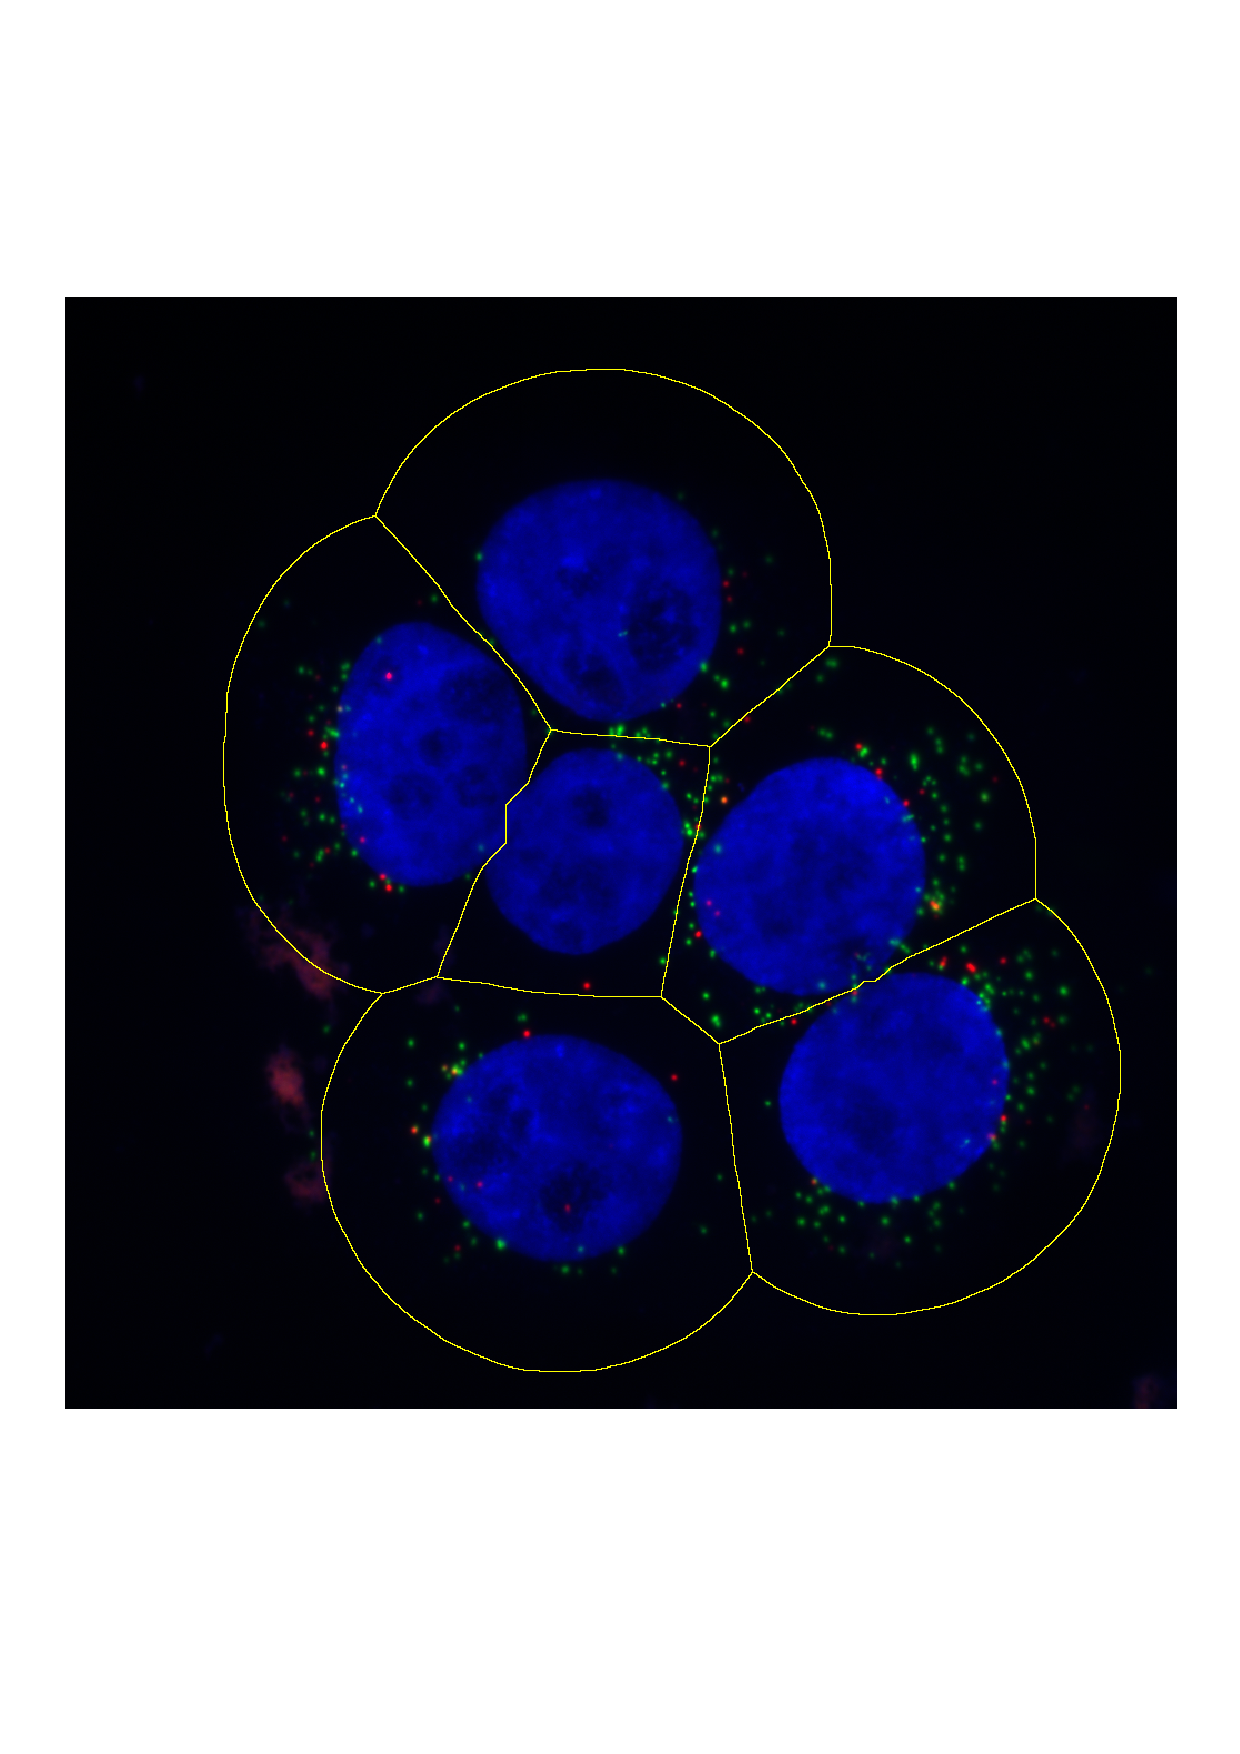
\includegraphics[width=0.6\textwidth]{Bilder/CellLines.pdf}
\caption{Lines inserted in to original image.}
\label{fig:CellLines}
\end{figure}


\end{document}
